\newpage
\section*{\centerline{Часть 2}}
	\paragraph{1)}
	Цель работы:  \\

	1) Изучение команд для просмотра типа файлов и содержимого файлов. \\

	2) Изучение команд для управления правами доступа к файлам и каталогам. \\

	3) Изучение команд для ввода/вывода данных. Перенаправление ввода/вывода. \\
	\subsection*{5 Просмотр содержимого файлов}
	
		\paragraph{1)}
		Цель: Просмотреть тип файлов из папки «Произведение автора» и файла, который извлекли из архива .zip (п.3 задания 2).\\

	 	Для просмотра типа файла можно использовать несколько вариантов команд, 		одни из 			которых \textit{file <name>} и \textit{file} с ключом 			\textit{--mime-type} . Для 			поиска файлов в папке Произведения 				Лермонтова воспользуемся формой \textit{./				Произведения\ 				Лермонтова/*} , где * обозначает любой файл. ( см. Рисунок 24, 25)
	\\
	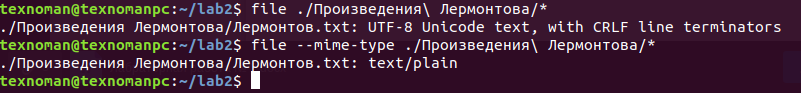
\includegraphics[width=\textwidth]{110.png} %из Произведения Лермонтова%
		\centerline{Рисунок 24 - просмотра типа файла при помоши \textit{file}}
	\\
	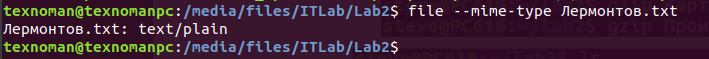
\includegraphics[width=\textwidth]{111.png} %из Lab2%
		\centerline{Рисунок 25 - просмотра типа файла при помоши \textit{file --mime-type}}

		\paragraph{2)}
		Цель: Просмотреть величину файлов. Выбрать наименьший пригодный для вывода на экран файл. Воспользоваться редактором cat. Вывести на экран содержимое файла, сжав пустые строки и пронумеровав строки с текстом (Использовать одну команду).\\

		Для просмотра величины файла была выбрана команда \textit{ls -s <name>}, 		где ключ \textit{-s} означает size. \\ 
	Выбирать особо не из чего, поэтому был выбран файл \textit{Лермонтов.txt}. (см. Рисунок 26) \\
	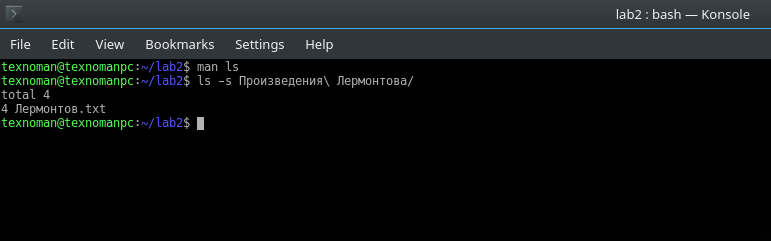
\includegraphics[width=\textwidth]{picture20.png}\\ 
		\centerline{Рисунок 26 - просмтр величины файла с использованием \textit{ls -s}}\\

		Далее, чтобы вывести текст на экран без пустых строк использовалась команда 	\textit{cat -b <(grep ' ' <name>)}, где \textit{-b} отображает номер строк, 		стрелка потока обозначает последовательность действий, а операция в  				\textit{grep} не дает возможность отображению пустых страк, так как в них 			отсутствуют знаки пробела.  (см. Рисунок 27)\\
	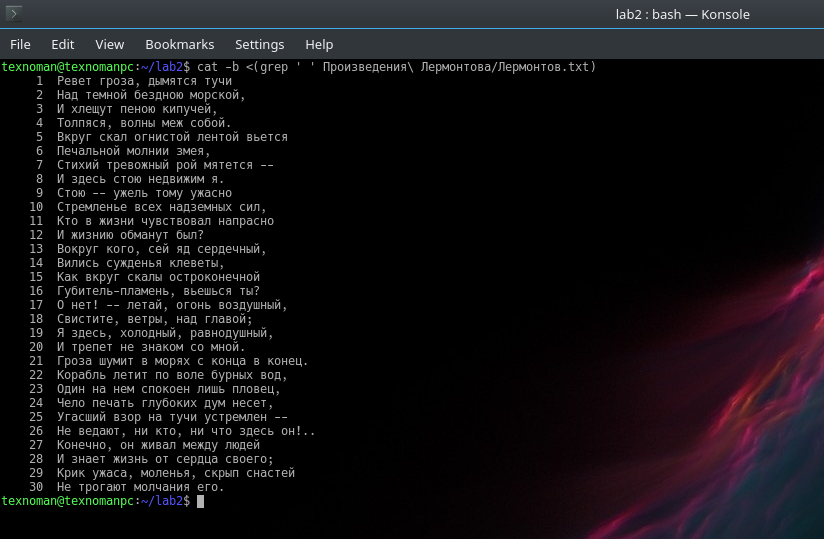
\includegraphics[width=\textwidth]{picture21.png}\\
		\centerline{Рисунок 27 - использование \textit{grep} для сжатия пустых строк}

		\paragraph{3)}
		Цель: Вывести любое произведение автора с помощью редактора more. Отобразить полуэкран (11 строк) текста из файла и вывести номер текущей строки (одной командой).\\

		За неимением других вариантов было выбрано произведение "Гроза". Для вывода 	первых 11 строк с помощью команды \textit{more} следует добавить \textit{-11}.  (см. Рисунок 28)
	\\
	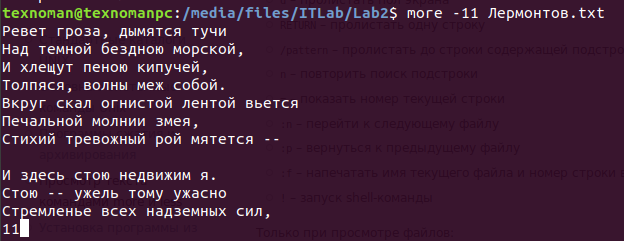
\includegraphics[width=\textwidth]{112.png}\\
		\centerline{Рисунок 28 - Использование \textit{more}, вывод первых 11 строк}

		\paragraph{4)}
		Цель: Выведите этот же текст, используя редактор less. \\

		Для вывода текста стихотворения с использованием \textit{less} вводим 			\textit{less <name>}  (см. Рисунок 29, 30)\\
	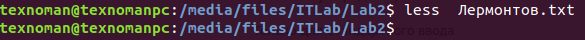
\includegraphics[width=\textwidth]{113(b).png}\\
		\centerline{Рисунок 29 - использование команды \textit{less}}


	\begin{center}
		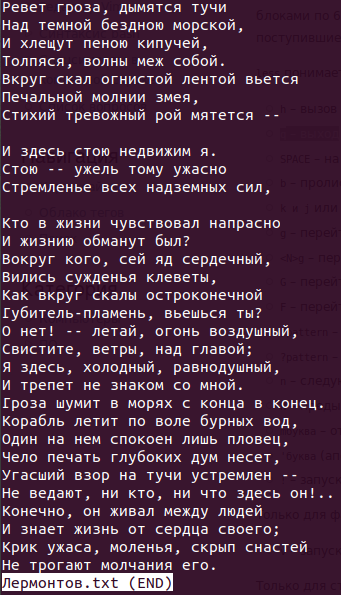
\includegraphics[width=\textwidth]{113(r).png}\\
			\centerline{ Рисунок 30 - результат работы \textit{less}}

	\end{center}
	
		\paragraph{5)}
		Цель: Проанализируйте отличия этих редакторов.\\

		В качестве анализа редакторов \textit{more} и \textit{less} можно 				предоствавить различия в просмотре документа: в дополнение к функциям 				\textit{more}  (постраничная или построчная прокрутка текста от начала до конца 	и поиск), команда less позволяет выполнять следующие операции: переход на 			указанную строку(number+g), переход в начало или  конец текста(g/G), прокрутка 		текста от конца к началу, поиск в обратном направлении.\\
		
	\subsection*{6 Управление правами доступа к файлам и каталогам}
	
		\paragraph{1)}
		Цель: Вывести полную информацию обо всех файлах из папки «Произведение автора» и файла, извлеченного из архива .zip (п.3 задания 2), и проанализировать выведенную информацию.\\
		
		Поскольку в 3 пункте 2 задания мы извлекали один файл, о нём и пойдет речь. 	Используем \textit{stat <name>} для вывода полной информации о файле.(см. Рисунок 31) \\
	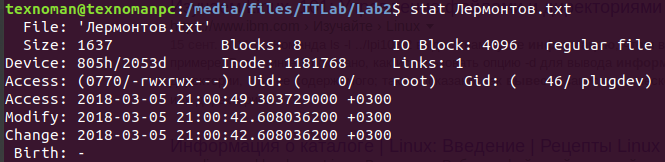
\includegraphics[width=\textwidth]{114.png}\\
		\centerline{Рисунок 31 - вывод полной информации о файле, используя \textit{state}}

	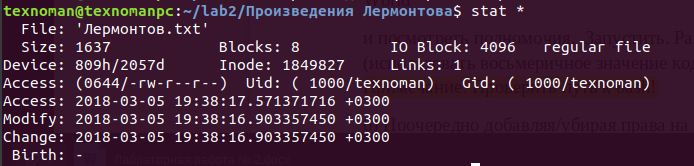
\includegraphics[width=\textwidth]{115.png}\\
		\centerline{Рисунок 32 - вывод полной информации о всех файлах, используя \textit{state}}

		\paragraph{2)}
		Цель: Удалить права на чтение в одном из произведений. Попытаться вывести на экран. 
		Проанализировать результат.\\

		Удаляем права на чтение в файле Лермонтов.txt, для 			этого вводим \textit{chmod a-r <name> }, где \textit{a-r} означает удаление(-) 		прав у всех (all)  пользователей на чтение (read). Мы не смогли прочесть файл (вывести текст на экран), это связанно с тем, что право на чтение файла было удалено для всех. 
		Прав нет - сделать нельзя. Результат анализа работы \textit{chmod} можно увидеть на Рисунке 33\\
	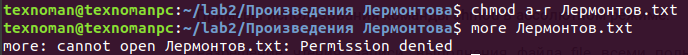
\includegraphics[width=\textwidth]{116.png}\\q
		\centerline{Рисунок 33 - удаление прав на чтение}

		\paragraph{3)}
		Цель: Удалить права на запись в одном из произведений. Попытаться внести изменения в текст. Проанализировать результат.\\

		Удаляем у файла Лермонтов.txt права на запись. Чтобы это сделать пишем: 		\textit{chmod a-w}, где \textit{a-w} - удалить(-) у всех(all) право на 				запись(write). Проверяем попыткой заменить пробемы на ничего, то есть удалить 		пробелы в тексте произведения. Pедактирование выбранного файла не получилось, потому что ранее были удалены права на изменение. Результат анализа работы \textit{chmod} можно увидеть на Рисунке 34\\
	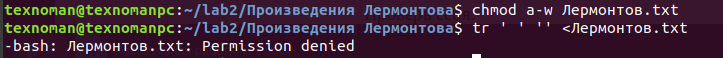
\includegraphics[width=\textwidth]{117.png}\\
		\centerline{Рисунок 34 - удаление прав на запись}

	
		\paragraph{4)}
		Цель: Добавить право выполнения членам группы и остальным пользователям для одного из текстов. Запустить. Проанализировать результат.\\

		Добавляем право выполнения членам группы и остальным  для документа 			Лермонтов.txt . Для этого используем команду \textit{chmod go+x}. Go(group and 		others) +(добавить) x(execute). Мы не можем 'выполнять' файл, поскольку не являемся группой пользователей и/или 'остальными', что можно видеть на изображение.(см. Рисунок 35) \\
	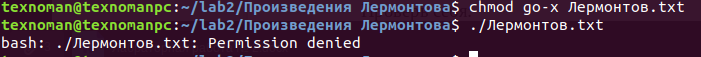
\includegraphics[width=\textwidth]{118.png}\\
		\centerline{Рисунок 35 - добавление права выполнения группе и остальным пользователям}

		\paragraph{5)}
		Цель: Создать текстовый файл hello\_world.sh с текстом: \#!/bin/bash echo "Hello World"\\

и посмотреть полномочия. Запустить. Разрешить файлу исполнение (использовать восьмеричное значение кода права доступа). Запустить. Примечание: Проверить путь к bash! 
	\\
		Для проверки местоположения bash нужно использовать вывод через echo переменной окружения \textit{\$SHELL}
		Создаём текстовый файл hello\_ world.sh с помощью редактора nano: 				\textit{nano}, прописываем текст \#!/bin/bash echo "Hello World", сохраняем и 		выходим. Выполняем проверку - всё работает, ехууу)) Проверяем путь - вcё хорошо.		\\
	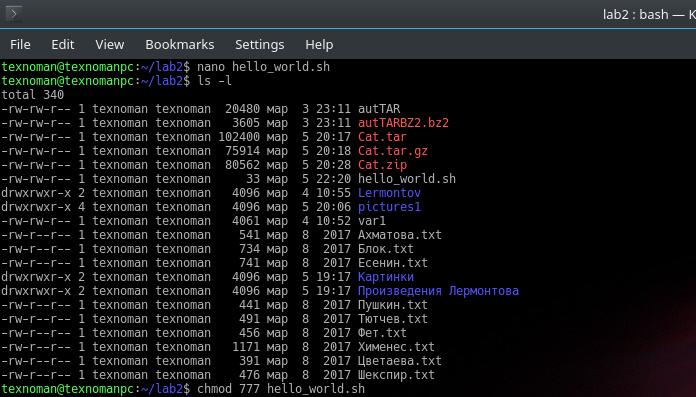
\includegraphics[width=\textwidth]{picture24.png}\\
		\centerline{Рисунок 36 - создение скрипта hello world на bash}

	\begin{center}
		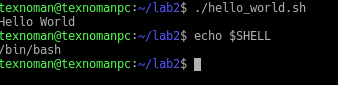
\includegraphics[width=\textwidth]{picture25.png}\\
			\centerline{(Рисунок 37 - запуск исполняемого файла,проверка пути к Bash}

	\end{center}
	
		\paragraph{6)}
		Поочередно меняем значения записи/чтения/выполнения, для чего используем 		\textit{chmod} в различные конфигурации. \\
		\textbf{Файл:}\\
		Для чтения нам требуется только право на чтение. Для записи права на запись (право на чтение не обязательно, если знаем название файла и его расположение, также право на использование не обязательно, если собственно использование избегать). Для удаления файла необходимо право на использование (опять же, если мы знаем название файла). Для перемещения и переименования анологично предыдущему описанию. Результат анализа изменения прав на файл можно увидеть на Рисунке 40\\
		\textbf{Директория:}\\
		Для копирования и перемещения директории необходимо наличие прав на запись \textit{w}, Рисунок 39.
		Для просмотра содержимого директории необходимы права на чтение. Оно используется для \textit{ls}, Рисунок 38.
		Права на исполнение \textit{X} для директории влияют на редактирование и запись файлов.

		
		\begin{center}
			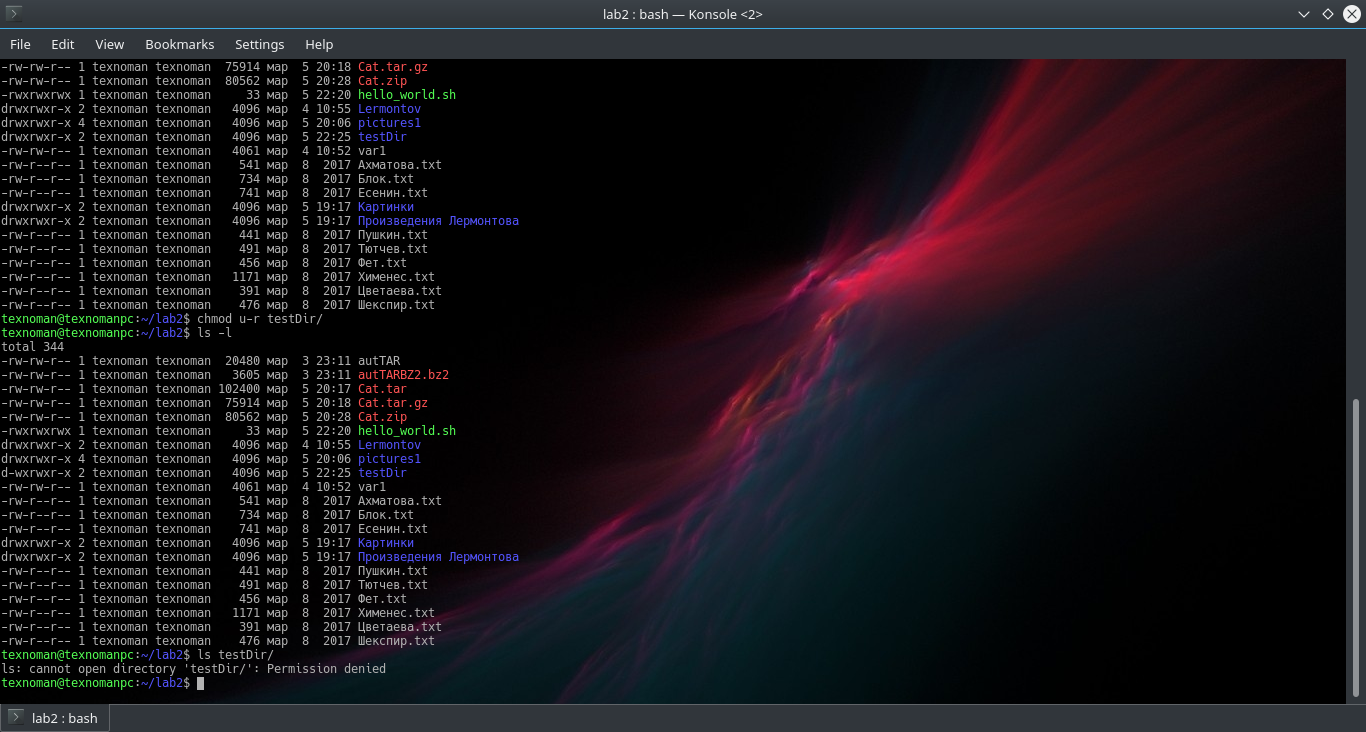
\includegraphics[width=\textwidth]{picture26.png}\\
				\centerline{(Рисунок 38 - удаление прав на чтение у директории}
		\end{center}
		\vspace{0.1cm}
		\begin{center}
			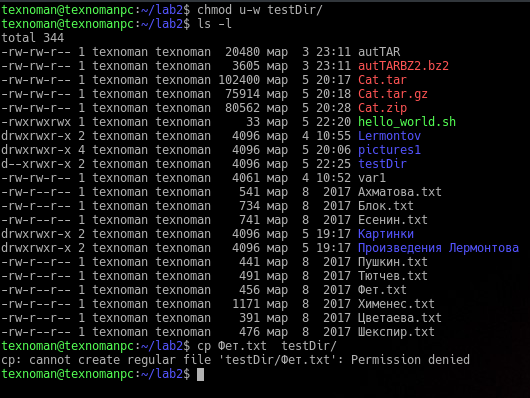
\includegraphics[width=\textwidth]{picture27.png}\\
				\centerline{(Рисунок 39 - удаление прав на запись у директории}
		\end{center}

		\begin{center}
			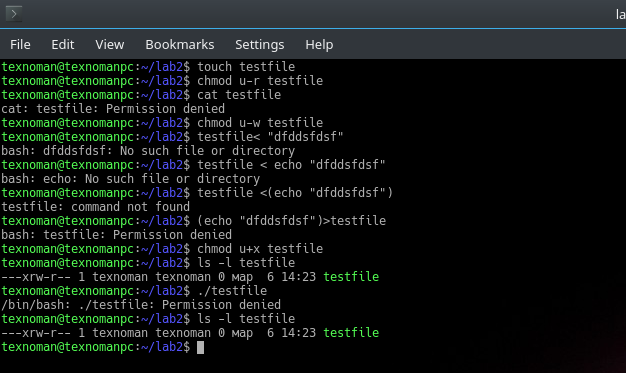
\includegraphics[width=\textwidth]{picture30.png}\\
				\centerline{Рисунок 40 - работа с правами у файла}
		\end{center}


	  
	  
	  
		